\section{Background}
\label{sec:background}
The work in this paper falls within the field of natural language grounding, which addresses the problem of correctly determining how phrases relate to the real world (e.g., the phrase ``go to the cube'' means approaching a physical cube).
% Before proceeding further, one must define the domains over which the grounding problem may be solved.
In the general formulation of the grounding problem, three sets must be considered: ${\Gamma = \{\text{symbolic actions and objects\}}}$ is the set of groundings, which represents what phrases may be grounded to; ${\Lambda = \{\text{English phrases}\}}$ is the set of phrases, which represents what phrases natural language sentences may be composed of; and ${\Upsilon = \Gamma^O \times \{\text{object attributes}\} }$ is the cartesian product of the set of objects (i.e., $\Gamma^O \subset \Gamma$) and the object attributes (e.g., color, location), which represents the world model in which the phrases may be grounded. 

Given a natural language command $\boldsymbol{\lambda}$, which is a vector of phrases from the set $\Lambda$ and has a length of $|\boldsymbol{\lambda}|$, 
%\indent Using these domains, it is possible to formulate 
the general grounding problem can be formulated as a probability maximization problem%, shown in Equation~\ref{eq:max_ground_prob},
\begin{equation}
\boldsymbol{\gamma}^* = \argmax_{\boldsymbol{\gamma} \in \Gamma^{|\boldsymbol{\lambda}|}} p(\boldsymbol{\gamma}|\boldsymbol{\lambda},\Upsilon),
\label{eq:max_ground_prob}
\end{equation}
where $\boldsymbol{\gamma} \in \Gamma^{|\boldsymbol{\lambda}|}$ is a vector of groundings with a length of $|\boldsymbol{\lambda}|$, and $\Upsilon$ denotes the world model. 
%$\gamma \in \Gamma$, $\boldsymbol{\lambda}$ as a vector of phrases $\lambda \in \Lambda$ and world model $\Upsilon$. 
In this formulation, the optimal vector of groundings $\boldsymbol{\gamma}^*$ is the one with maximum likelihood, given a command $\boldsymbol{\lambda}$ and a world model $\Upsilon$.

In practice, the domains of $\Gamma$, $\Lambda$, and $\Upsilon$ in \eqref{eq:max_ground_prob} typically include elements from previously seen examples. % While the general formulation allows any possible grounding, phrase, or world model, the domains of $\Gamma$, $\Lambda$, and $\Upsilon$ are shrunk in existing solutions to the grounding problem.
For example, rather than allowing the set of phrases $\Lambda$ to include all words in a dictionary, $\Lambda$ is generally assumed to only contain words that have appeared in the training examples. Moreover, solving \eqref{eq:max_ground_prob} is a hard combinatorial optimization problem due to the diversity in language and world.
% even though limited sets ($\Gamma$, $\Lambda$, and $\Upsilon$) are considered. 
One way to tackle this issue is to construct probabilistic graphical models based on the linguistic structure of the commands. For example, the Generalized Grounding Graph (G3) model \cite{g3} is a factor graph that is trained from a corpus of labeled examples to ground language commands with objects, locations, and paths.  

An alternative model is the Distributed Correspondence Graph (DCG) \cite{dcg}, which infers the most likely set of planning constraints from language commands (rather than grounding phrases to particular actions, objects, or paths as in G3 model). In particular, the DCG model has the following properties:  
First, the DCG decouples motion planning from the grounding problem. To this end, it discards the notion of grounding to specific actions or objects by instead only grounding to constraints relative to known objects (e.g. the area near a cube). Then, it passes the constraints to a motion planner.
Second, the DCG allows only the phrases composed entirely of the words that have already been encountered in training.
Third, the DCG only considers the perceived objects rather than a full model of the world including the unobserved objects.
Fourth, ternary correspondence variables $\phi_{ij}$ are introduced to represent whether the $i^\text{th}$ phrase $\lambda_i$ from the overall command $\boldsymbol{\lambda}$ corresponds to a grounding $\gamma_{ij}$.
For a given phrase $\lambda_i$, $\phi_{ij}$ is set to \emph{Active} if $\lambda_i$ refers to constraint $\gamma_{ij}$ (e.g., the area near the cube), \emph{Inverted} if $\lambda_i$ refers to the opposite of $\gamma_{ij}$ (e.g. the area far from the cube), or \emph{Inactive} if $\lambda_i$ has no bearing on $\gamma_{ij}$ (e.g. the area near a sphere).
Fifth, for the sake of computational efficiency, the overall inference is factored using conditional independence according to the structure of the parse tree of $\boldsymbol{\lambda}$.

Accordingly, the optimization problem solved over a DCG model becomes
\begin{equation}
\label{eq:dcg_factored1}
\begin{split}
\boldsymbol{\phi}^* = \argmax_{\phi_{ij} \in \boldsymbol{\phi}} \prod_{i}^{|\boldsymbol{\lambda}|} \prod_{j}^{|\Phi_i|} p(\phi_{ij}|\gamma_{ij},\lambda_i,\Gamma_{c_{ij}} , \Upsilon_{KP}),
\end{split}
\end{equation}
where $\lambda_i \in \Lambda_{KN}$ is the $i^{th}$ phrase in command $\boldsymbol{\lambda}$ and $\Lambda_{KN}$ is the set of phrases with known (previously seen) words; $\Phi_i$ is the set of correspondence variables of $\lambda_i$, $\phi_{ij} \in \Phi_i$ is the $j^{th}$ correspondence variable of $\lambda_i$; $\gamma_{ij}$ is the $j^{th}$ grounding of $\lambda_i$; $\Upsilon_{KP} = \{\text{object attributes}\} \times \Gamma_{KP}$ is the world model consisting of the object attributes and the set of known perceived symbolic objects $\Gamma_{KP}$; and  $\Gamma_{c_{ij}}$ is the set of child groundings of $\gamma_{ij}$. Note that $\Gamma_{c_{ij}}$ is defined as the set of groundings for the immediate children phrases (leftmost descendants) of the parent phrase $\lambda_i$ in the parse tree of the natural language command.

For example, consider Fig.~\ref{fig:parse_tree} that shows the parse tree of a simple command, and Fig.~\ref{fig:dcg_plates} that shows the corresponding DCG graphical model. The child grounding of the phrase ``move'' is the grounding for the phrase ``to.'' Similarly, the child grounding of the phrase ``to'' is the grounding for the phrase ``the cube'' (determiners such as ``the'' may be collapsed into their nouns). Thus, in this example, each grounding has exactly one child grounding, yielding the inter-plate structure in Fig.~\ref{fig:dcg_plates}.
Examining the parse tree also reveals why the factorization in \eqref{eq:dcg_factored1} is reasonable: the meaning ``move'' should be conditionally independent of the noun ``cube'' given the prepositional phrase.
After all, the correct grounding of the word ``move'' is an action that does not depend on whether the target is a cube or a sphere, but it does depend on the position of the cube.
%Finally, the domains are redefined for $\gamma \in C=\{\text{Constraints}\}$, $\lambda \in \Lambda_{KN}=\{\text{phrases with known nouns}\}$, and $\Upsilon \in \{\text{object attributes}\} \times \Gamma_{KP}$ for $\Gamma_{KP} = \{\text{known perceived symbolic objects}\}$.\\
%\indent As stated previously, DCG assumes conditional independence among groundings, given $\Gamma_{c_{ij}}$.
%Child groundings $\Gamma_{c_i}$ may be formally defined as the set of groundings for the leftmost descendants of the immediate children (barring itself) of the parent of phrase $i$ in the parse tree of the natural language command.


\begin{figure}[b!]
\centering
\begin{subfigure}[b]{0.39\columnwidth}
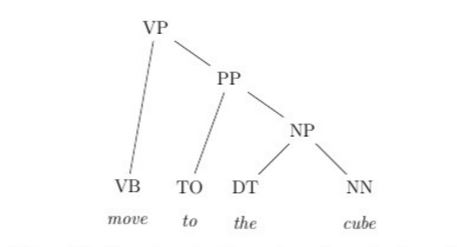
\includegraphics[width=\textwidth]{parse_tree}
\caption{Parse tree for the command ``move to the cube''}
\label{fig:parse_tree}
\end{subfigure}
~
\begin{subfigure}[b]{0.55\columnwidth}
\centering
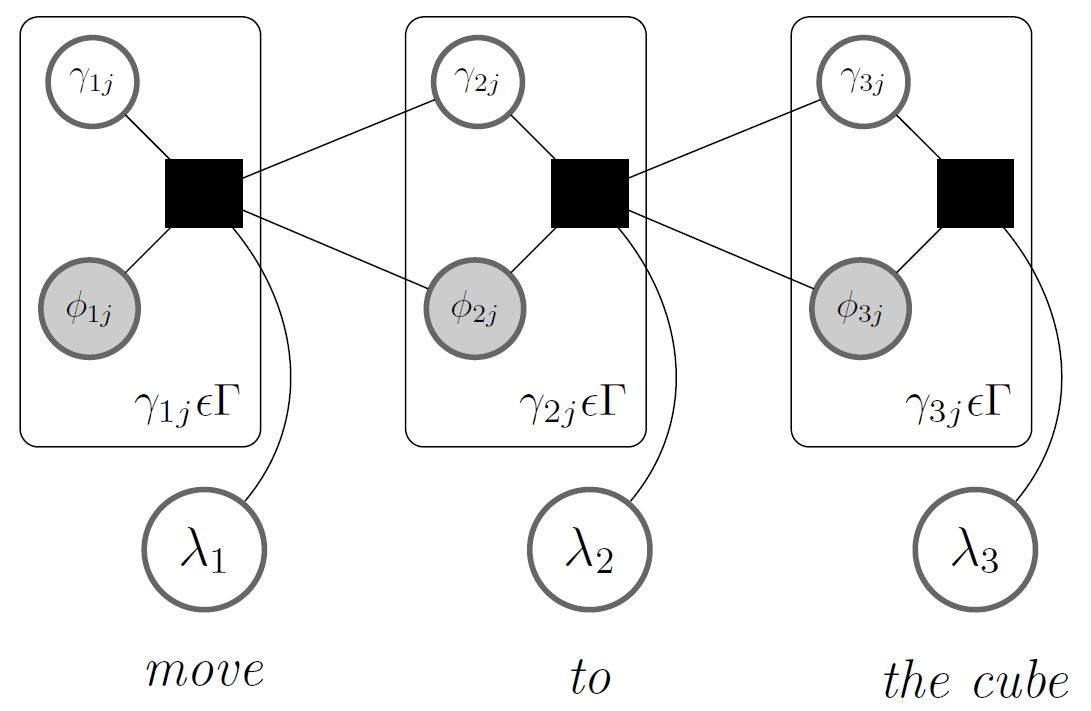
\includegraphics[width=\textwidth]{dcg_plates}
\caption{The DCG graphical model for the parse tree in Fig.~\ref{fig:parse_tree}}
\label{fig:dcg_plates}
\end{subfigure}
\caption{An illustration of a parse tree and the corresponding DCG model.}
\end{figure}

Finally, one must consider the factor function $\Psi : \Phi \times \Gamma \times \Lambda \times \Gamma \times \Upsilon \rightarrow
 \mathbb{R}$ within each plate that determines the most likely configuration of each $\phi_{ij} \in \Phi$ given $\gamma_{ij} \in \Gamma$, $\lambda_i \in \Lambda$, $\Gamma_{c_{ij}} \subset \Gamma$, and $\Upsilon_{KP} \subset \Upsilon$. Accordingly, one may rewrite \eqref{eq:dcg_factored1} as
%In order to expose the use of $\Psi$, one may rewrite Equation~\ref{eq:dcg_factored1} as Equation~\ref{eq:llm1}, \\
\begin{equation}
\boldsymbol{\phi}^* = \argmax_{\phi_{ij} \in \boldsymbol{\phi}} \prod_{i}^{\boldsymbol{|\lambda|}} \prod_{j}^{|\Phi_i|} \Psi(\phi_{ij},\gamma_{ij},\lambda_i,\Gamma_{c_{ij}},\Upsilon_{KP}),
\label{eq:llm1}
\end{equation}
where $\Psi$ is a log-linear model (LLM) composed of a weighted combination of hand-coded binary functions, that is,
\begin{equation}
\Psi(\phi_{ij},\gamma_{ij},\lambda_i,\Gamma_{c_{ij}},\Upsilon_{KP}) = \frac {\exp \Big( \sum\limits_{f \epsilon F} \mu_f f(\phi_{ij},\gamma_{ij},\lambda_i,\Gamma_{c_{ij}},\Upsilon_{KP}) \Big)}{\sum\limits_{\phi_{ij} \in \{-1,0,1\}}\exp \Big( \sum\limits_{f \epsilon F} \mu_f f(\phi_{ij},\gamma_{ij},\lambda_i,\Gamma_{c_{ij}},\Upsilon_{KP}) \Big)},
\label{eq:llm2}
\end{equation}
where each binary function $f$ belongs to a set of hand-coded binary features that evaluate specific traits about a grounding (e.g., whether the word ``cube'' appears in $\boldsymbol{\lambda}$), and $\mu_f$ is the weighting of each $f$. In this work,
the weights $\mu_f$ are learned in a training procedure via the Limited-memory Broyden-Fletcher-Goldfarb-Shanno algorithm.% to generate a more nuanced function that evaluates how likely a phrase is to correspond to a grounding.